    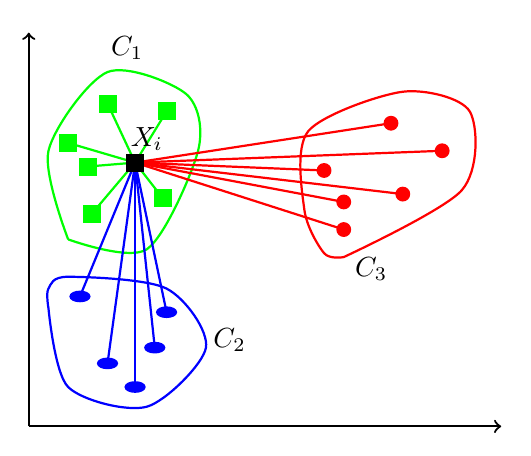
\begin{tikzpicture}[scale=1.0]

    % green cluster
%    \draw[thick,color=green,fill=green] (0.8,2.7) circle (0.07);
%%    \draw[thick,color=green,fill=green] (1.0,3.0) circle (0.07);
%    \draw[thick,color=green,fill=green] (1.7,2.9) circle (0.07);%%%
%    \draw[thick,color=black,fill=black] (1.35,3.35) circle (0.07);%%%%% x_i
%    \draw[thick,color=green,fill=green] (0.75,3.3) circle (0.07);
%    \draw[thick,color=green,fill=green] (1.75,4.0) circle (0.07);
%    \draw[thick,color=green,fill=green] (0.5,3.6) circle (0.07);
%    \draw[thick,color=green,fill=green] (1.0,4.1) circle (0.07);
    \draw[thick,color=green,fill=green] (0.7,2.6) rectangle (0.9,2.8);
%    \draw[thick,color=green,fill=green] (0.9,2.9) rectangle (1.1,3.1);
    \draw[thick,color=green,fill=green] (1.6,2.8) rectangle (1.8,3.0);%%%
    \draw[thick,color=green,fill=green] (0.65,3.2) rectangle (0.85,3.4);
    \draw[thick,color=green,fill=green] (1.65,3.9) rectangle (1.85,4.1);
    \draw[thick,color=green,fill=green] (0.4,3.5) rectangle (0.6,3.7);
    \draw[thick,color=green,fill=green] (0.9,4.0) rectangle (1.1,4.2);

    % blue cluster
%    \draw[thick,color=blue,fill=blue] (1.75,1.45) circle (0.07);
%    \draw[thick,color=blue,fill=blue] (1.0,0.8) circle (0.07);
%    \draw[thick,color=blue,fill=blue] (0.65,1.65) circle (0.07);
%    \draw[thick,color=blue,fill=blue] (1.6,1.0) circle (0.07);
%    \draw[thick,color=blue,fill=blue] (1.35,0.5) circle (0.07);
    \draw[thick,color=blue,fill=blue] (1.75,1.45) ellipse (0.12 and 0.06);
    \draw[thick,color=blue,fill=blue] (1.0,0.8) ellipse (0.12 and 0.06);
    \draw[thick,color=blue,fill=blue] (0.65,1.65) ellipse (0.12 and 0.06);
    \draw[thick,color=blue,fill=blue] (1.6,1.0) ellipse (0.12 and 0.06);
    \draw[thick,color=blue,fill=blue] (1.35,0.5) ellipse (0.12 and 0.06);

    % red cluster
    \draw[thick,color=red,fill=red] (4.0,2.5) circle (0.08);
%    \draw[thick,color=red,fill=red] (4.25,2.1) circle (0.08);
    \draw[thick,color=red,fill=red] (4.75,2.95) circle (0.08);
    \draw[thick,color=red,fill=red] (5.25,3.5) circle (0.08);
%    \draw[thick,color=red,fill=red] (4.75,3.0) circle (0.08);
    \draw[thick,color=red,fill=red] (4.0,2.85) circle (0.08);
    \draw[thick,color=red,fill=red] (3.75,3.25) circle (0.08);%%%
    \draw[thick,color=red,fill=red] (4.6,3.85) circle (0.08);
%    \draw[thick,color=red,fill=red] (5.0,3.2) circle (0.08);

%    \draw[blue,thick] plot [smooth] coordinates {
%    (0.75,1.5) (1.0,0.5) (2.0,0.25) (2.75,1.0) (2.25,1.75) (1,1.9) (0.75,1.75) (0.75,1.5)};
    \draw[blue,thick] plot [smooth] coordinates {
    (0.25,1.5) (0.5,0.5) (1.5,0.25) (2.25,1.0) (1.75,1.75) (0.5,1.9) (0.25,1.75) (0.25,1.5)};
    \draw[red,thick] plot [smooth] coordinates {
    (4.0,2.15) (5.5,3.0) (5.6,4.0) (4.75,4.25) (3.55,3.75) (3.5,2.75) (3.75,2.2) (4.0,2.15)};
    \draw[green,thick] plot [smooth] coordinates {
    (0.5,2.375) (1.5,2.25) (2.15,3.5) (2.0,4.22) (1.0,4.5) (0.25,3.5) (0.5,2.375)};
        
    \draw[thick,color=green] (1.35,3.35) -- (0.8,2.7);
    \draw[thick,color=green] (1.35,3.35) -- (1.7,2.9);%%%
    \draw[thick,color=green] (1.35,3.35) -- (0.75,3.3);
    \draw[thick,color=green] (1.35,3.35) -- (1.75,4.0);
    \draw[thick,color=green] (1.35,3.35) -- (0.5,3.6);
    \draw[thick,color=green] (1.35,3.35) -- (1.0,4.1);

    \draw[thick,color=blue] (1.35,3.35) -- (1.75,1.45);
    \draw[thick,color=blue] (1.35,3.35) -- (1.0,0.8);
    \draw[thick,color=blue] (1.35,3.35) -- (0.65,1.65);
    \draw[thick,color=blue] (1.35,3.35) -- (1.6,1.0);
    \draw[thick,color=blue] (1.35,3.35) -- (1.35,0.5);

    \draw[thick,color=red] (1.35,3.35) -- (4.0,2.5);
    \draw[thick,color=red] (1.35,3.35) -- (4.75,2.95);
    \draw[thick,color=red] (1.35,3.35) -- (5.25,3.5);
    \draw[thick,color=red] (1.35,3.35) -- (4.0,2.85);
    \draw[thick,color=red] (1.35,3.35) -- (3.75,3.25);%%%
    \draw[thick,color=red] (1.35,3.35) -- (4.6,3.85);

    \draw[thick,color=black,fill=black] (1.25,3.25) rectangle (1.45,3.45);%%%%% x_i

    % grid (aid to plotting)
%    \draw[step=0.5,gray,very thin] (0,0) grid (5,5);
        
    % axes
    \draw[thick,color=black,->] (0,0) -- (6,0); % x axis
    \draw[thick,color=black,->] (0,0) -- (0,5); % y axis
   
    \node at (1.5,3.65){$X_i$};
%    \node at (1.25,4.8){$a = \avg_1$};
    \node at (1.25,4.8){$C_1$};
    \node at (2.55,1.1){$C_2$};
    \node at (4.35,2.0){$C_3$};
%    \node[rotate around={-55:(2.25,2.5)}] at (2.25,2.5){$b_1 = \mu_e$};
%    \node[rotate around={-55:(2.25,2.5)}] at (3.35,0.2){$b_1 = \mu_e$};
%    \node at (2.4,2.05){$b_1 = \avg_2$};
%    \node[rotate around={2.5:(2.75,2.75)}] at (2.75,2.75){$b_2 = \mu_c$};
%    \node at (2.75,2.60){$b_2 = \mu_c$};
%    \node at (2.9,3.90){$b_2 = \avg_3$};
%    \node at (4.35,1.10){$b = \min(b_1,b_2)$};

    \end{tikzpicture}
